\label{chapter:Methods and Materials}
In this project, we have used NodeMCU, an Ultrasonic sensor, Firebase real-time database, and an SMTP mail function.

\section{Analysis}
One of the main function of our project is e-mail notification. As there are several mail transfer protocols such as SMTP(Simple Mail Transfer Protocol), POP(Post Office Protocol), and IMAP(Internet Message Access Protocol), we have find best method for mail transfer. 

\subsection{Comparison of SMTP, POP, and IMAP}
The Simple Mail Transfer Protocol (SMTP) is a protocol that mail servers use to send, receive, and/or relay email between senders and receivers. The address (or addresses) of an SMTP email server can be set by the mail client or application you're using, and is usually formatted as smtp.serveraddress.com.

The most significant distinction between these protocols is that SMTP is the only protocol that allows you to transmit, or "push," email from one unknown mail server to another. POP and IMAP are email protocols for receiving or "pulling" messages from a recipient's own mail server. As a result, POP and IMAP only allow mail to be sent to confirmed mail servers. They can't be used outside of your own networks for communication \cite{Goud2020}.

POP is a message access protocol, whereas SMTP is a message transfer protocol. To put it another way, SMTP is used to transmit mail from one user to another, and POP is used to receive mail. SMTP is used twice: once to establish the connection and send data between the sender and the email server, and again to send data and connect to the receiver. Between the receiver and their mail server, POP is only utilized once \cite{Tzerefos1997}.

IMAP is a message access protocol, whereas SMTP is a message transfer protocol. IMAP simply fetches messages and handles incoming email, whereas SMTP transmits messages and handles outgoing email \cite{kara2019}.

With SMTP, we will receive helpful delivery information regardless of what happens to your email after you send it. You can check to verify if your messages were sent to the intended recipient and look for any problem codes \cite{Bettina2022}.

Another benefit of running your own SMTP is that email list is not being shared with anyone, ensuring the data privacy of company and customer \cite{Bettina2022}.

\section{Modelling}
\subsection{Modelling Post Detection}
Modeling is used to obtain the desired functionality of the Post detecting system. The smart postal mailbox is a system for determining the presence of posts in a mailbox from a remote location regardless of distance, consisting of a sensor for detecting the presence of post in a mailbox, while the sensor is positioned in the mailbox; a control unit that communicates with the mailbox sensor and is used for storing information of the mailbox status, while the status is used for observation. Following are the most signification functions:
\begin{itemize}
    \item detecting the presence of a consignment in the mailbox
    \item collecting time data about deliveries,
    \item storing data in the database,
    \item ensuring communication between database and NodeMCU
\end{itemize}

\subsection{Modelling User Notification}
The real-time mail alert system is a device that helps users by providing real-time notifications when new mail arrives, replacing the usual method of monitoring mail. User will get notified, with aid of header file 'ESP\textunderscore Mail\textunderscore Client.h' and implementing SMTP mail function.

\section{Tools and Technologies}
In the creation of this real-time post box notification, we employed the following hardware, and Technologies which is listed below.

\subsection{NodeMCU ESP8266}
A microcontroller unit, which is a small computer, is housed on a single metal-oxide-semiconductor integrated circuit chip. A microcontroller is a device with one or more CPUs, memory, and programmable input/output peripherals that can be used to connect miniature screens, buttons, motors, and sensors, among other things. A microcontroller may be programmed and controlled. The microcontroller's primary duty is to connect to WiFi and then to the Firebase. The microcontroller has been configured to connect to both WiFi and the Firebase. As a result, the data from the ultrasonic sensor is used to compare the distances, and an event is triggered in the Firebase as a result \cite{Shakthidhar2019}.
\begin{figure}[htp]
    \centering
    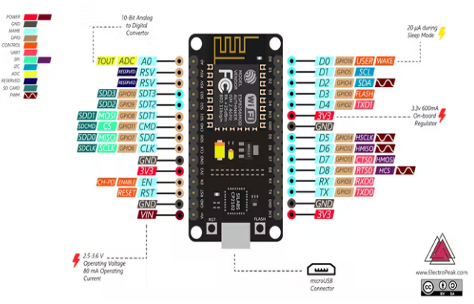
\includegraphics[width=12cm]{image/NodeMCU.png}
    \caption{NodeMCU \cite{NodeMCUIMG}.}
    \label{fig:NodeMCU}
\end{figure}

\subsection{HC-SR04 Sensor (Ultrasonic Sensor)}
The HC-SR04 is a low-cost, simple-to-use distance measuring sensor with a range of 2 to 400 cm (about an inch to 13 feet). Two ultrasonic transducers make up the sensor. One is the transmitter, which generates ultrasonic sound pulses, and the other is the receiver, which detects reflected waves. You may compute the distance by taking into account the travel time and the sound's speed. The Trig pin must be set to High State for 10 seconds in order to create the ultrasonography. This will cause an 8-cycle ultrasonic burst to be sent out, which will travel at the speed of sound. After those 8 cycles, an ultrasonic burst is sent, the Echo pins go high right immediately, and it begins listening or waiting for that wave to be reflected from an item. If no object or reflected pulse is present, the Echo pin will time out after 38 milliseconds and return to its low state. The Echo pin will travel down faster than those 38ms if we receive a reflected pulse. We can determine the distance traveled by the sound wave based on the length of time the Echo pin was HIGH, and thus the distance from the sensor to the item \cite{Dimitrov2016}.
\begin{figure}[htp]
    \centering
    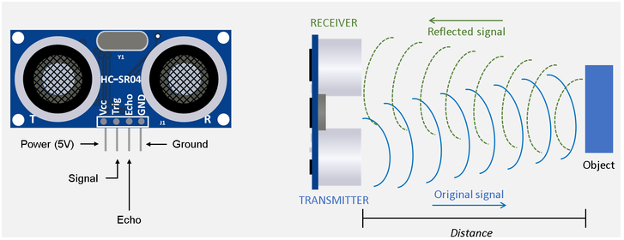
\includegraphics[width=12cm]{image/ultrasonic_sensor.png}
    \caption{Ultrasonic sensor \cite{ultrasonicIMG}.}
    \label{fig:ultrasonic}
\end{figure}

\subsection{Firebase Database}
Firebase, which is owned by Google, is a real-time database stored on the cloud. It distributes a real-time database instance to each connected client and ensures that they receive real-time updates with the most recent data. It saves data in JSON format and allows for cross-platform scripting. In terms of the scope of our prototype, it saves all users' unique IDs, login credentials, device state information, and usage duration \cite{Moroney2017}.

\section{Implementation}
In our project we have implemented hardware as well as software side in form of cloud database and email function.
\subsection{Hardware Implementation}
The hardware implementation of the system is very straightforward, as it has only two components, one is NodeMCU, and another is an ultrasonic sensor.

First of all, an ultrasonic sensor is connected to NodeMCU. Trigger pin and Echo pin are connected to two GPIO of NodeMCU and ground and Vcc are connected with its related pin.

After that, NodeMCU is connected with a remote power supply such as a 9V battery or power bank. 
\begin{figure}[htp]
    \centering
    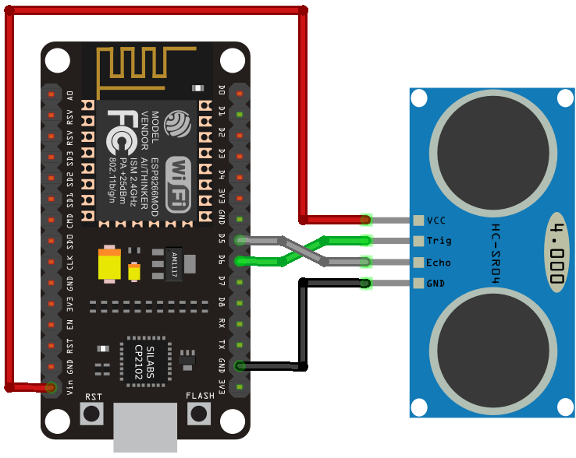
\includegraphics[width=10cm, height=8cm]{image/Circuit_diagram.png}
    \caption{Circuit diagram}
    \label{fig:circuit_diagram}
\end{figure}

\subsection{Software Implementation}
The Software side of our project includes mainly Firebase database and SMTP mail function.

\textbf{Firebase Implementation}, we have created a new database with relevant fields along with a distance field, which is most important because this field will be updated every time the post-box receives a new post.

\textbf{Distance Function}, it measures the distance between the sensor and the post-box door. A limit is set to 8. The Trig (Trigger) pin triggers the ultrasonic sound pulses. The echo pin generates a pulse when it receives the reflected signal. Based on the measured duration distance variable is calculated. 

\textbf{Storing real-time data}, for this we must include header file 'FirebaseESP8266.h' to connect NodeMCU to the Firebase. The variables used and seen in Fig.~\ref{fig:firebaseauth} are: 
\begin{itemize}
    \item API\textunderscore KEY - identify your Firebase project
    \item DATABASE\textunderscore URL – URL of the database
    \item USER\textunderscore EMAIL – Email of user’s Firebase account
    \item USER\textunderscore PASSWORD – Password of user’s Firebase account
\end{itemize}

\begin{figure}[htp]
    \centering
    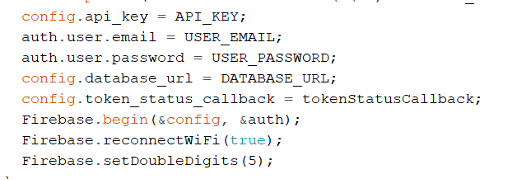
\includegraphics[width=12cm]{image/firebase-auth.png}
    \caption{Snippet - Firebase auth}
    \label{fig:firebaseauth}
\end{figure}

\textbf{Notifying users}, the user will get notified by email when a new post arrives in the post-box. For this, we set a predefined condition, if the distance is less than 8 then using the SMTP mail function user will get notified by email. A header file that should be included for the mail function is ESP\textunderscore Mail\textunderscore Client.h. The variables used are: 
\begin{itemize}
    \item SMTP\textunderscore HOST- Server name
	\item SMTP\textunderscore PORT - A communication endpoint that handles the transfer of email data over SMTP 
	\item AUTHOR\textunderscore EMAIL – Sender’s email address
	\item AUTHOR\textunderscore PASSWORD – Sender’s password for the particular email address
	\item RECIPIENT\textunderscore EMAIL – Receiver’s email address.
\end{itemize}

Fig.~\ref{fig:SMTPmail} shows a code snippet for notifying the users by email regarding the new arrival of post.
\begin{figure}[htp]
    \centering
    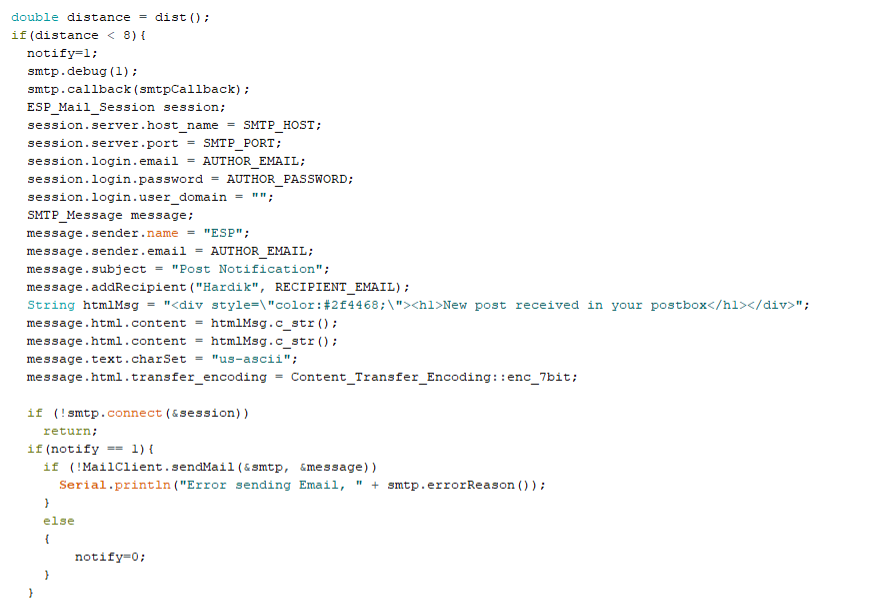
\includegraphics[width=14cm, height=13cm]{image/SMTP_mail.png}
    \caption{Snippet - SMTP mail}
    \label{fig:SMTPmail}
\end{figure}

\section{Flow Diagram}

First of all, we initialize the ultrasonic sensor by providing power. Now ultrasonic sensor transmits rays and distance will be calculated frequently. If the distance is less than 8 that means a new post arrived in the post-box and NodeMCU sends this distance data to Firebase and stores it there. After this SMTP mail function gets called and the user gets a notification about the arrival of a new post. Otherwise, it measures distance continuously. 
\begin{figure}[htp]
    \centering
    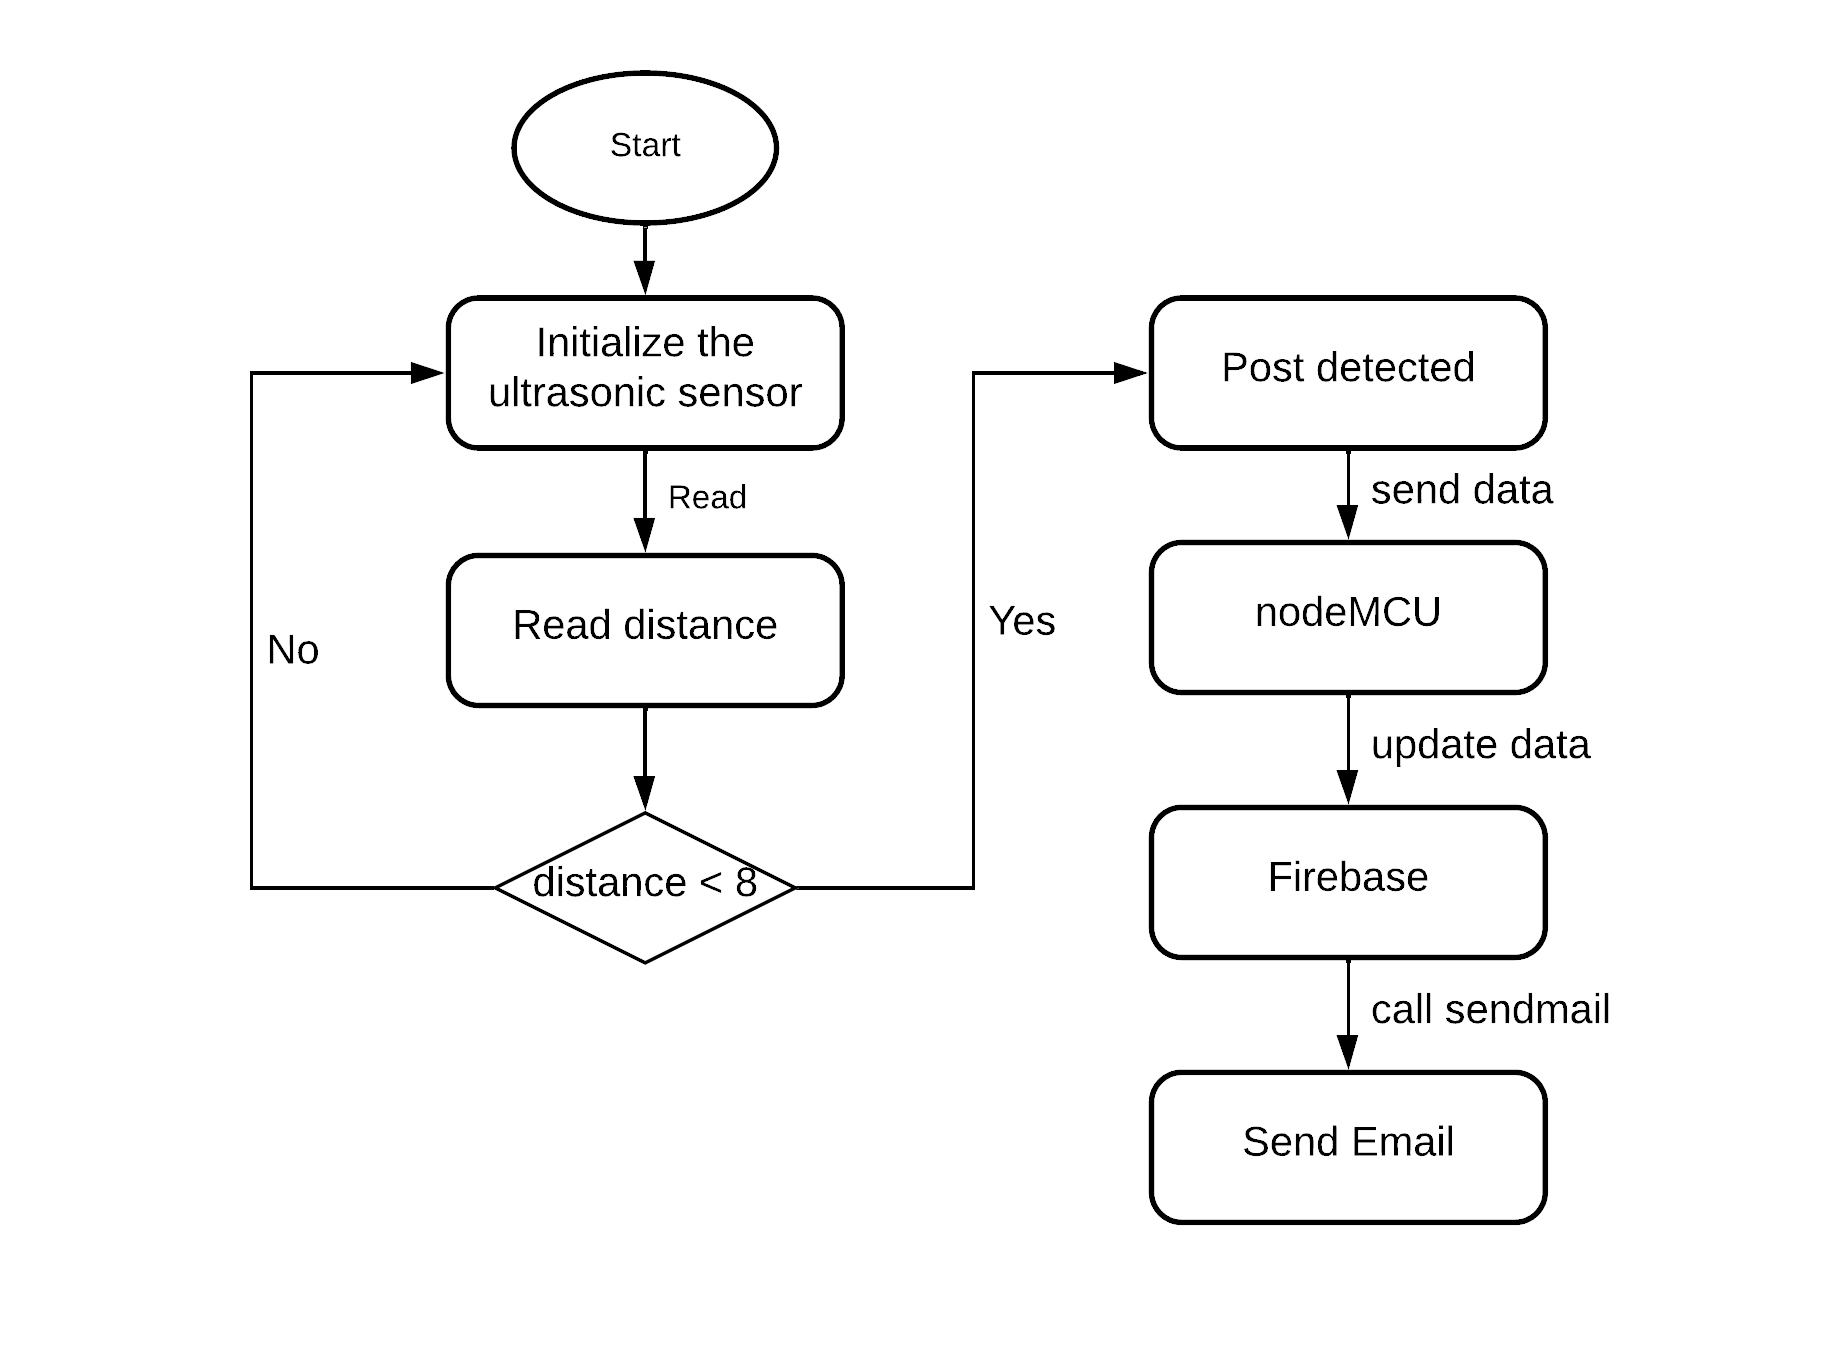
\includegraphics[width=12cm]{image/HCI.png}
    \caption{Snippet - SMTP mail}
    \label{fig:Flowchart}
\end{figure}\\
We have uploaded the source code along with a video of the running prototype, and source code of Latex on GitHub. \textbf{\href{https://github.com/hardik1111/Real-Time-Postbox-Notification}{https://github.com/hardik1111/Real-Time-Postbox-Notification}}:
